\documentclass{misisarticle}
\usepackage{graphicx}
\usepackage{booktabs}
\usepackage{array}
\usepackage{url}
\usepackage{placeins} % для ограничения перемещения плавающих объектов
\usepackage{float} % для размещения рисунков и таблиц рядом с текстом
\title{НЕЙРОННЫЕ СЕТИ ДЛЯ РАСПОЗНАВАНИЯ И КЛАССИФИКАЦИИ 3D-ОБЪЕКТОВ}
\misisauthor{Л. Б. Комендала}{кафедра инженерной кибернетики НИТУ «МИСиС»}{Москва, Россия}{m2517795@edu.misis.ru}
\setabstract{В настоящее время трехмерные данные активно используются в робототехнике, автономных транспортных системах, промышленной автоматизации, а также в технологиях виртуальной и дополненной реальности. Одной из ключевых задач компьютерного зрения является распознавание и классификация 3D-объектов. Современные методы глубокого обучения позволяют эффективно решать данную задачу благодаря автоматическому извлечению признаков из трехмерных данных. В данной работе проводится сравнительный анализ двух популярных нейронных сетей — PointNet и VoxNet. Для проведения экспериментов используется датасет ModelNet40. Выполнено сравнение моделей по точности классификации и времени инференса. Полученные результаты позволяют определить преимущества и недостатки каждого подхода и сформулировать рекомендации по их практическому применению.}
\setkeywords{компьютерное зрение, глубокое обучение, PointNet, VoxNet, ModelNet40, облака точек, воксельные сети, классификация 3D-объектов}
\begin{document}
\maketitle
\section{ВВЕДЕНИЕ}
Развитие технологий искусственного интеллекта и компьютерного зрения привело к значительному росту интереса к обработке трехмерных данных. В отличие от традиционных двумерных изображений, 3D-модели содержат информацию о пространственной структуре объекта, что делает их особенно полезными для робототехники, автономной навигации и систем дополненной реальности [1].\par
Распознавание и классификация 3D-объектов представляет собой важную задачу, направленную на автоматическое определение принадлежности объекта к определенному классу. Ранее для решения подобных задач использовались методы ручного извлечения признаков, однако современные методы глубокого обучения позволяют автоматически выделять информативные характеристики объектов и обеспечивать высокую точность классификации [1].\par
\section{НАБОРЫ ДАННЫХ}
\subsection{ModelNet40}
Для проведения основного эксперимента используется датасет ModelNet40 [6], который является одним из наиболее распространенных наборов данных для оценки алгоритмов классификации трехмерных объектов. Датасет содержит 12311 CAD-моделей, распределенных по 40 категориям объектов. Набор включает 9843 объекта для обучения и 2468 объектов для тестирования.\par
К основным категориям относятся самолеты, автомобили, столы, стулья, кровати, шкафы и другие объекты повседневного использования. Благодаря разнообразию классов ModelNet40 широко используется для сравнения современных методов обработки трехмерных данных.\par
\begin{figure}[H]
\centering
\begin{minipage}[t]{0.48\columnwidth}
  \centering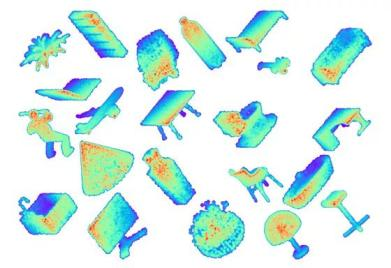
\includegraphics[width=\linewidth]{figures/image1.jpeg}
\end{minipage}\hfill
\begin{minipage}[t]{0.48\columnwidth}
  \centering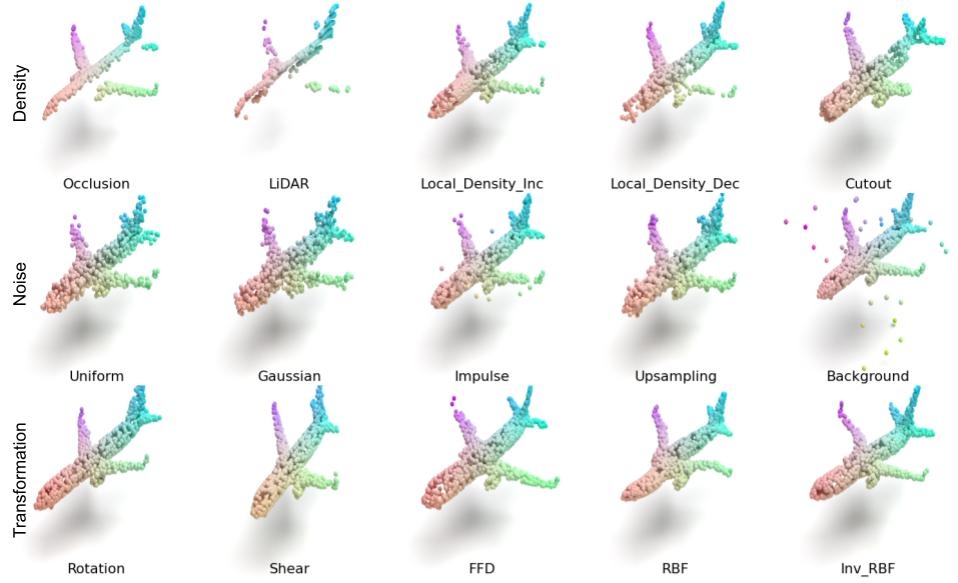
\includegraphics[width=\linewidth]{figures/image2.jpeg}
\end{minipage}\par\vspace{2mm}
\begin{minipage}[t]{0.48\columnwidth}
  \centering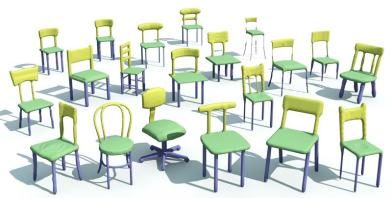
\includegraphics[width=\linewidth]{figures/image3.jpeg}
\end{minipage}\hfill
\begin{minipage}[t]{0.48\columnwidth}
  \centering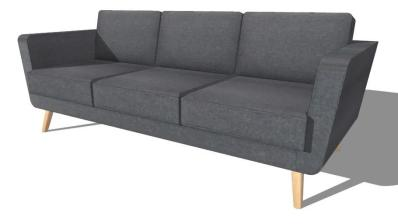
\includegraphics[width=\linewidth]{figures/image4.jpeg}
\end{minipage}
\caption{Примеры трёхмерных объектов из набора данных ModelNet40.}
\label{fig:modelnet-examples}
\end{figure}
\begin{table}[H]
\centering
\small
\caption{Характеристики набора данных ModelNet40}
\label{tab:modelnet40}
\begin{tabular}{|p{0.55\columnwidth}|p{0.30\columnwidth}|}
\hline
Параметр & Значение \\ \hline
Количество классов & 40 \\ \hline
Общее число моделей & 12311 \\ \hline
Обучающая выборка & 9843 \\ \hline
Тестовая выборка & 2468 \\ \hline
Формат данных & OFF \\ \hline
\end{tabular}
\end{table}
\FloatBarrier
\section{НЕЙРОСЕТЕВЫЕ АРХИТЕКТУРЫ}
\subsection{PointNet}
PointNet представляет собой архитектуру глубокого обучения, предназначенную для непосредственной обработки облаков точек без преобразования их в регулярную структуру данных [1]. Входными данными сети является множество точек, описывающих поверхность трехмерного объекта. В рамках данного исследования для каждого объекта используется облако из 1024 точек.\par
Архитектура сети состоит из нескольких многослойных перцептронов (MLP), которые применяются независимо к каждой точке. Далее выполняется операция симметричной агрегации признаков с использованием слоя Max Pooling, что обеспечивает инвариантность сети к перестановке точек во входном облаке.\par
После извлечения глобального признакового вектора используются полносвязные слои (Fully Connected Layers), выполняющие окончательную классификацию объекта.\par
Основными этапами обработки данных в PointNet являются:\par
входное облако точек (1024 точки);\par
многослойный перцептрон (MLP);\par
операция Max Pooling;\par
полносвязные слои (Fully Connected Layers);\par
выходной слой классификации.\par
\begin{figure}[H]
\centering
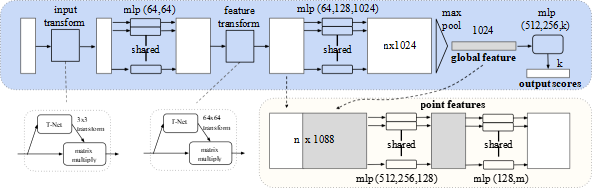
\includegraphics[width=0.92\columnwidth]{figures/image5.png}
\caption{Архитектура нейронной сети PointNet [1].}
\label{fig:pointnet}
\end{figure}
Преимуществом PointNet является возможность непосредственной обработки облаков точек без необходимости преобразования данных в воксельное представление, что снижает вычислительные затраты и объем используемой памяти.\par
B.VoxNet\par
VoxNet представляет собой архитектуру глубокой нейронной сети, предназначенную для классификации трехмерных объектов на основе воксельного представления данных [2]. В отличие от PointNet, работающего непосредственно с облаками точек, VoxNet использует регулярную трехмерную сетку (voxel grid), в которой объект представляется набором заполненных и пустых вокселей.\par
Перед подачей данных на вход сети трехмерная модель преобразуется в воксельную сетку фиксированного размера, например 32×32×32. Такое представление позволяет применять трехмерные сверточные операции аналогично обработке двумерных изображений в классических сверточных нейронных сетях.\par
Архитектура VoxNet включает следующие основные компоненты:\par
входной слой с воксельной сеткой;\par
трехмерные сверточные слои (3D Convolutional Layers);\par
функции активации ReLU;\par
слои объединения признаков (Pooling);\par
полносвязные слои (Fully Connected Layers);\par
выходной слой классификации.\par
Процесс работы сети начинается с извлечения локальных пространственных признаков при помощи трехмерных сверток. Далее полученные признаки агрегируются и передаются в полносвязные слои, выполняющие окончательную классификацию объекта.\par
Основным преимуществом VoxNet является способность эффективно учитывать пространственную структуру объекта и извлекать локальные геометрические признаки. Однако использование воксельного представления приводит к увеличению потребления памяти и вычислительных ресурсов по сравнению с методами, работающими непосредственно с облаками точек.\par
\begin{figure}[H]
\centering
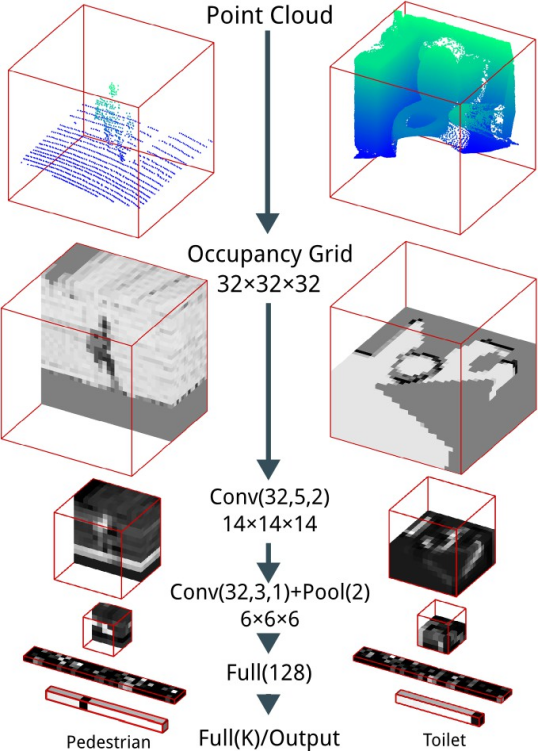
\includegraphics[width=0.92\columnwidth]{figures/image6.png}
\caption{Архитектура нейронной сети VoxNet [2].}
\label{fig:voxnet}
\end{figure}
\begin{table}[H]
\centering
\small
\caption{Сравнение архитектур PointNet и VoxNet}
\label{tab:pointnet-voxnet}
\begin{tabular}{|p{0.30\columnwidth}|p{0.30\columnwidth}|p{0.30\columnwidth}|}
\hline
Характеристика & PointNet & VoxNet \\ \hline
Входные данные & Облако точек & Воксельная сетка \\ \hline
Тип сети & MLP & 3D CNN \\ \hline
Представление данных & Нерегулярное & Регулярное \\ \hline
Извлечение локальных признаков & Ограниченное & Эффективное \\ \hline
\end{tabular}
\end{table}
\FloatBarrier
Таким образом, PointNet и VoxNet представляют два различных подхода к классификации трёхмерных объектов: PointNet непосредственно обрабатывает облако точек, а VoxNet использует воксельное представление и трёхмерные свёртки. В проведённом эксперименте PointNet показала более высокие значения Accuracy и взвешенной F1-меры, а также меньшее среднее время инференса. Эти выводы относятся к использованной подвыборке из 629 объектов и указанным условиям эксперимента.\par
\FloatBarrier
\section{ЭКСПЕРИМЕНТАЛЬНОЕ ИССЛЕДОВАНИЕ}
\subsection{Подготовка данных}
Для проведения эксперимента использовался набор данных ModelNet40 [6], содержащий 12 311 CAD-моделей 40 классов. В стандартном разделении набора 9843 объекта относятся к обучающей выборке, а 2468 — к тестовой. В данном исследовании качество классификации оценивалось на подвыборке из 629 тестовых объектов, выбранной для сокращения времени эксперимента и вычислительных затрат. Для корректного сравнения PointNet и VoxNet необходимо использовать один и тот же набор тестовых объектов. Способ формирования подвыборки в имеющемся описании не указан, поэтому этот аспект следует уточнить по исходному коду или журналам эксперимента.\par
Для PointNet трехмерные модели были преобразованы в облака точек. Из каждого объекта случайным образом выбиралось 1024 точки в соответствии с рекомендациями авторов архитектуры PointNet [1].\par
Для VoxNet трехмерные модели были преобразованы в воксельные сетки размером 32×32×32, что соответствует подходу, предложенному в работе Maturana и Scherer [2].\par
Настройка обучения\par
Модели реализованы с использованием библиотеки PyTorch [4]. В описании эксперимента не указаны число эпох, размер пакета, оптимизатор, скорость обучения, способ выбора контрольной выборки и характеристики аппаратной платформы. Эти параметры следует добавить по фактическим настройкам кода или журналам запуска; без них воспроизведение эксперимента затруднено.\par
\subsection{Метрики оценки}
Для оценки качества классификации использовались Accuracy, Precision, Recall и F1-score [5]. Accuracy отражает долю правильных предсказаний среди всех объектов. Precision показывает, какая доля объектов, отнесённых моделью к определённому классу, действительно принадлежит этому классу; Recall характеризует долю правильно найденных объектов данного класса. F1-score является гармоническим средним Precision и Recall. Для агрегированных значений Precision, Recall и F1-score необходимо указать способ усреднения по классам (macro, micro или weighted), соответствующий фактически использованному коду.\par
\subsection{Среда выполнения эксперимента}
Обучение моделей выполнялось с использованием современных методов глубокого обучения, реализованных средствами библиотеки PyTorch [4].\par
Для PointNet значение Precision составило 75,53\%, а взвешенная F1-мера — 73,38\%. Для VoxNet соответствующие показатели составили 60,37\% и 64,99\%.\par
Несмотря на близкие значения Accuracy, между моделями наблюдается заметное различие в Precision и взвешенной F1-мере. Это показывает, что общая точность не всегда полностью отражает качество классификации по отдельным категориям.\par
В частности, низкое значение взвешенной Precision модели VoxNet указывает на наличие ошибочных положительных предсказаний. Однако для установления причин таких ошибок необходимо дополнительно исследовать распределение предсказаний по классам.\par
Использование нескольких метрик является важным условием комплексной оценки классификаторов: Precision характеризует долю правильных предсказаний среди объектов, отнесённых к определённому классу, Recall — долю правильно обнаруженных объектов этого класса, а F1-score объединяет Precision и Recall в одну метрику.\par
Таким образом, результаты эксперимента показывают необходимость анализа не только общей точности, но и ошибок классификации отдельных категорий.\par
\subsection{Анализ матриц ошибок}
Для изучения особенностей классификации моделей используются матрицы ошибок (confusion matrices), позволяющие определить распределение правильных и ошибочных предсказаний по отдельным классам.\par
Для PointNet матрица ошибок отражает результаты классификации объектов, представленных облаками точек. Такой подход соответствует исходной концепции архитектуры, предложенной Qi и соавторами [1].\par
Для VoxNet матрица ошибок позволяет оценить результаты классификации объектов, представленных воксельными сетками, с использованием трёхмерных свёрточных операций [2].\par
Сравнение матриц ошибок позволяет определить категории, которые распознаются успешно, а также классы, между которыми возникают систематические ошибки. Особое внимание следует уделить категориям с низкими значениями Precision, Recall и F1-score.\par
\begin{figure}[H]
\centering
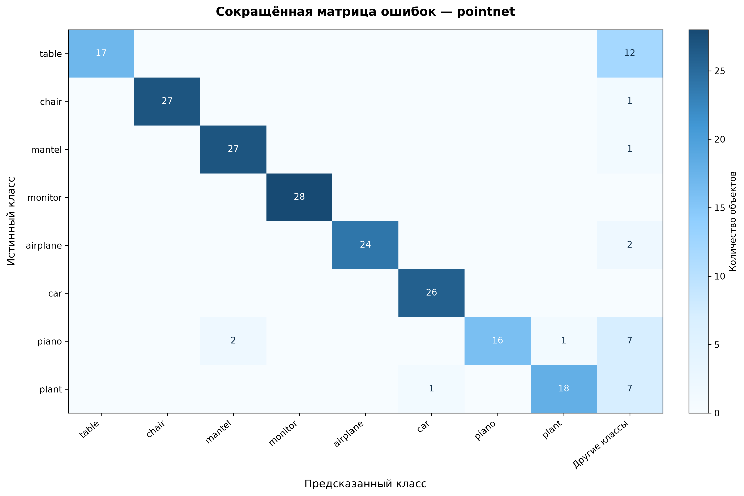
\includegraphics[width=0.92\columnwidth]{figures/image7.png}
\caption{Матрица ошибок модели PointNet.}
\label{fig:cm-pointnet}
\end{figure}
\begin{figure}[H]
\centering
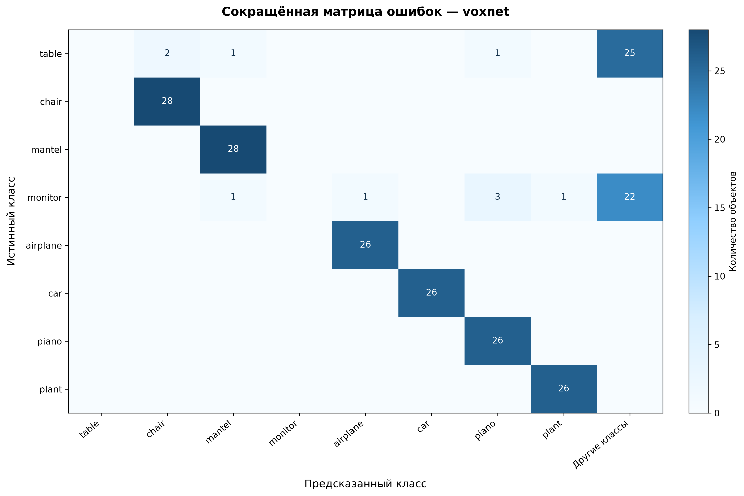
\includegraphics[width=0.92\columnwidth]{figures/image8.png}
\caption{Матрица ошибок модели VoxNet.}
\label{fig:cm-voxnet}
\end{figure}
\subsection{Сравнение вычислительной эффективности}
Дополнительно оценивалась скорость инференса моделей. Общее время инференса PointNet составило 4,674 с, а среднее время обработки одного объекта — 7,43 мс. Для VoxNet общее время составило 7,474 с, а среднее время обработки одного объекта — 11,88 мс.\par
Таким образом, в рамках данного измерения PointNet обрабатывал один объект приблизительно в 1,60 раза быстрее, чем VoxNet.\par
Данное наблюдение согласуется с различиями в способах представления данных. PointNet непосредственно обрабатывает наборы трёхмерных точек [1], тогда как VoxNet использует объёмное представление и трёхмерные свёрточные операции [2]. Однако фактическая скорость инференса зависит не только от архитектуры, но и от аппаратной платформы, реализации моделей, размера пакета данных и особенностей предварительной обработки.\par
Поэтому полученные значения характеризуют производительность реализованных моделей в условиях проведённого эксперимента и не должны рассматриваться как универсальное сравнение всех возможных реализаций PointNet и VoxNet.\par
Следует отметить, что в рамках текущей оценки измерялось время инференса. Для полноценного сравнения вычислительных затрат необходимо отдельно измерить время обучения и потребление памяти обеими моделями.\par
\subsection{Обсуждение результатов}
Результаты исследования демонстрируют различия между двумя подходами к классификации трёхмерных объектов. PointNet был разработан для непосредственной обработки облаков точек с учётом инвариантности к перестановке точек во входном наборе [1]. VoxNet использует воксельное представление и трёхмерную свёрточную нейронную сеть для извлечения пространственных признаков объектов [2].\par
В проведённом эксперименте PointNet показал более высокие значения Accuracy, Precision и F1-score, а также меньшее время инференса. Разница в Accuracy составила 1,43 процентного пункта, а среднее время обработки одного объекта PointNet было приблизительно в 1,60 раза меньше, чем у VoxNet.\par
При этом разница в общей точности сравнительно невелика, тогда как различие во взвешенном F1-score более выражено. Это подчёркивает необходимость учитывать распределение ошибок между классами, а не ограничиваться одной метрикой.\par
Полученные результаты следует интерпретировать с учётом ограничений экспериментальной постановки. Перед формулированием окончательных выводов необходимо подтвердить соответствие предварительной обработки данных процедурам обучения обеих моделей и убедиться в отсутствии пересечения обучающей и тестовой выборок. Дополнительные эксперименты с несколькими случайными инициализациями позволят оценить устойчивость результатов.\par
В целом предварительные результаты показывают преимущество PointNet по измеренным метрикам в использованной конфигурации эксперимента. Окончательные выводы должны основываться на проверенной методологии, анализе матриц ошибок и, при необходимости, дополнительных экспериментах.\par
\FloatBarrier
\section{ЗАКЛЮЧЕНИЕ}
В данной работе было проведено сравнительное исследование нейронных сетей PointNet и VoxNet для классификации трёхмерных объектов на основе набора данных ModelNet40. Оценка моделей проводилась на подвыборке из 629 тестовых объектов, использованной для сокращения времени выполнения экспериментов и вычислительных затрат.\par
Согласно полученным экспериментальным результатам, PointNet продемонстрировала более высокую точность классификации по сравнению с VoxNet: 74,56 \% против 73,13 \%. Кроме того, значение взвешенной F1-меры для PointNet составило 73,38 \%, тогда как для VoxNet — 64,99 \%. В рамках проведённого эксперимента PointNet также показала меньшее среднее время обработки одного объекта: 7,43 мс по сравнению с 11,88 мс у VoxNet.\par
Таким образом, на использованной подвыборке PointNet показала лучшие результаты по точности классификации, взвешенной F1-мере и времени обработки одного объекта. Вместе с тем полученные результаты относятся к выбранной подвыборке из 629 объектов и не позволяют однозначно судить о качестве моделей на всей тестовой выборке ModelNet40, содержащей 2468 объектов. Для подтверждения выявленных различий целесообразно провести дополнительную оценку обеих моделей на полной тестовой выборке.\par
В рамках эксперимента на подвыборке из 629 тестовых объектов PointNet показала Accuracy 74,56\% и взвешенную F1-меру 73,38\%, тогда как для VoxNet соответствующие значения составили 73,13\% и 64,99\%. Среднее время инференса одного объекта составило 7,43 мс для PointNet и 11,88 мс для VoxNet. Следовательно, на использованной подвыборке PointNet обеспечила более высокие значения указанных метрик и меньшую задержку инференса. Поскольку оценка проводилась не на всей тестовой выборке ModelNet40, полученные результаты нельзя без дополнительной проверки переносить на все 2468 тестовых объектов. В дальнейшем следует провести оценку обеих моделей на полной тестовой выборке, указать способ формирования подвыборки и параметры обучения, а также проанализировать матрицы ошибок по классам.\par
\FloatBarrier
\section{ЛИТЕРАТУРА}
[1] Qi C. R., Su H., Mo K., Guibas L. J. PointNet: Deep Learning on Point Sets for 3D Classification and Segmentation // Proceedings of the IEEE Conference on Computer Vision and Pattern Recognition (CVPR). 2017. P. 652–660. DOI: 10.1109/CVPR.2017.16. URL: https://openaccess.thecvf.com/content\_cvpr\_2017/html/Qi\_PointNet\_Deep\_Learning\_CVPR\_2017\_paper.html\par
[2] Maturana D., Scherer S. VoxNet: A 3D Convolutional Neural Network for Real-Time Object Recognition // Proceedings of the IEEE/RSJ International Conference on Intelligent Robots and Systems (IROS). 2015. P. 922–928. DOI: 10.1109/IROS.2015.7353481. URL: https://publications.ri.cmu.edu/voxnet-a-3d-convolutional-neural-network-for-real-time-object-recognition\par
[3] Wu Z., Song S., Khosla A., Yu F., Zhang L., Tang X., Xiao J. 3D ShapeNets: A Deep Representation for Volumetric Shapes // Proceedings of the IEEE Conference on Computer Vision and Pattern Recognition (CVPR). 2015. P. 1912–1920. DOI: 10.1109/CVPR.2015.7298801.\par
[4] Paszke A. et al. PyTorch: An Imperative Style, High-Performance Deep Learning Library // Advances in Neural Information Processing Systems. 2019. Vol. 32. P. 8024–8035. URL: https://papers.nips.cc/paper\_files/paper/2019/hash/bdbca288fee7f92f2bfa9f7012727740-Abstract.html\par
[5] Pedregosa F. et al. Scikit-learn: Machine Learning in Python // Journal of Machine Learning Research. 2011. Vol. 12. P. 2825–2830. URL: https://www.jmlr.org/papers/v12/pedregosa11a.html\par
[6] Princeton Vision \& Robotics Group. ModelNet dataset. URL: https://modelnet.cs.princeton.edu/ (дата обращения: 22.10.2026).\par

\end{document}
